\begin{figure}[h!]
\centering
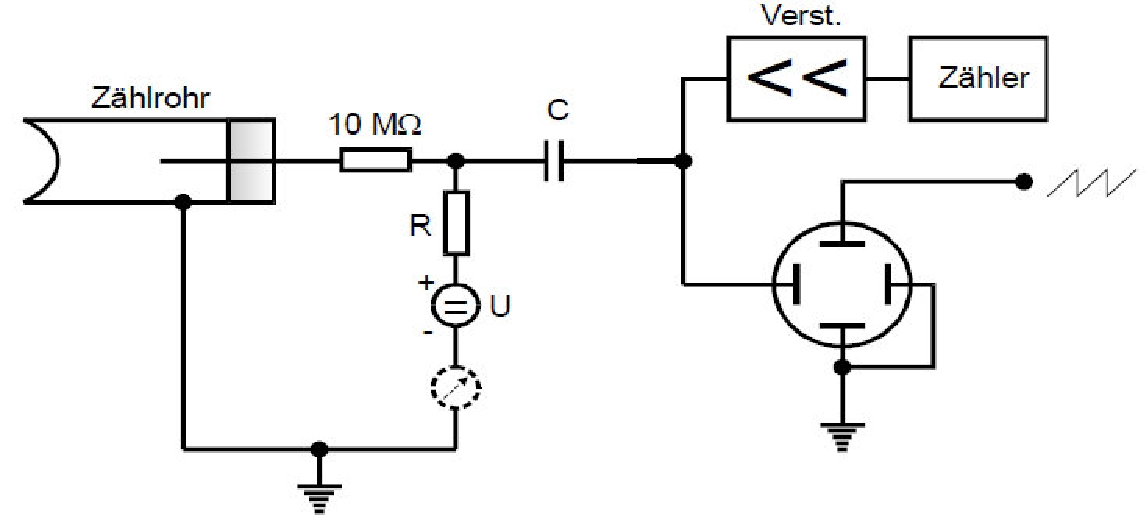
\includegraphics[scale=0.7]{Grafiken/Durchfuehrung.pdf}
\caption{Die verwendete Schaltung für den Versuch \cite{V703}}
\label{AB}
\end{figure}
In Abbildung \ref{AB} ist der schematische Aufbau zu sehen. Über den Widerstand $R$ fliest der Ladungsimpuls, der durch den Kondensator $C$ ausgekoppelt wird und durch den Verstärker und dem Zählgerät gemessen werden kann. Über ein Oszilloskop werden die Impulse sichtbar gemacht und in der internen Schaltung des Zählrohrs ist ein Mikroamperemeter mit dem der Strom gemessen werden kann.


\subsection{Messung der Charakteristik}
Es wird für eine $\beta$-Quelle die Abhängigkeit der Zählrate zur angelegten Spannung gemessen. Die Messzeit beträgt hier \SI{100}{\second}, damit der Fehler >1$\%$ beträgt. Die Spannung sollte bei diesem Geiger-Müller-Zählrohr nicht über \SI{700}{\volt} gehen.


\subsection{Messung der Nachentladung mithilfe des Oszilloskops}
Die Strahlintensität wird so weit abgesenkt, dass auf dem Oszilloskop nur ein Impuls zu sehen ist. Damit keine Nachentladungen auftreten, wird die Spannung auf \SI{350}{\volt} gestellt. Danach wird die Spannung auf \SI{700}{\volt} gestellt um den zeitlichen Abstand zwischen den Primär- und dem Nachentladungsimpuls zu messen.


\subsection{Messung der Totzeit mithilfe des Oszilloskops}
Für eine hohe Strahlenintensität wird die Totzeit gemäß Abbildung \ref{Totzeit} gemessen, dabei lässt sich die Erholungszeit nur grob abschätzen.


\subsection{Bestimmung der Totzeit durch die Zwei-Quellen-Methode}
Die registrierte Impulsrate $N_r$ ist immer kleiner als die wahre Impulsrate $N_W$, aufgrund der Totzeit $T$. Es lässt sich der Zusammenhang
$$
N_W=\frac{N_r}{1-T \, N_r}
$$
erkennen. Bei Verwendung von zwei Quellen, gilt aufgrund der Totzeit 
$$
N_{1+2}\, <\, N_1+N_2,
$$
ohne die Totzeit würde hier Gleichheit gelten. Hier raus lässt sich
\begin{align}
\label{eq:Theorie_Totzeit}
T\approx\frac{N_1+N_2-N_{1+2}}{2N_1N_2}
\end{align}
herleiten. Für das Experiment bedeutet das, es wird erst die Zählrate für eine Quelle gemessen, anschließend für zwei und danach noch ein mal nur für die zweite Quelle. Beim Ein- und Ausbauen der Quelle ist darauf zu achten, dass die Position der jeweils anderen Quelle nicht verändert wird.
\subsection{Messung der Ladungsmenge}
Mithilfe des eingebauten Mikroamperemeters kann der Strom in Abhängigkeit von der angelegten Spannung gemessen werden. Nach Definition für den mittleren Strom gilt
\begin{align}
\label{eq:Theorie_Ladungsmenge}
\overline{I}=\frac{\Delta Q}{\Delta t}Z.
\end{align}